\documentclass[../main.tex]{subfiles}

\begin{document}

\problem{1}

Using \(\frac{p_2}{p_2}\) as the metric for oblique-shock strength, come up with a way to graphically show the relationship between shock strength, \(\beta\), and \(M_{1,\infty}\).

\assumptions{}
Assume a weak, attached oblique shock for a range of \(\beta\) and \(M_{1,\infty}\) with \(\gamma=1.4\).
For all Machs analyzed, a max wave angle of \(60^\circ\) is below the strong shock solution.
Using  \(\beta_{min}=1/\arcsin{(M_{1,\infty})}\) ensures all solutions are physically possible for an attached, left-running shock.

\solution{}
\textit{Note: All calculations performed in Python, see appendix \ref{Problem1Python}.}\\
We examine a range of Mach numbers from 2-10 with wave angle \(\beta\) ranging from the minimum value (\(\beta_{min}=1/\arcsin{(M_{1,\infty})}\)) to \(60^\circ\).
Pressure ratios across the oblique shock are calculated using normal shock relations and the component of \(M_{1,\infty}\) normal to the wave angle:

\[
    \frac{p_2}{p_1}
    =
    1 + \frac{2}{\gamma+1}
    \left({
    M_{1,\infty}^2 \sin^2{\beta} - 1
    }\right)
\]

Figure \ref{pr_2d} shows a 2D scatterplot of pressure ratio versus wave angle for a series of Machs from 2-10.
Although shock strength does always increase with wave angle, the pressure ratio shows greater increases for an increase in Mach number.
Lower Mach flows cannot experience wave angles as small as higher Mach flows, as shown by the difference between the \(\beta_{min}\) for Mach 2 flow and Mach 10 flow (\(30^\circ\,\textrm{vs.}\,<1^\circ\)).
The greater sensitivity to freestream Mach number indicates that there is no contradictory behavior between normal shocks and oblique shocks.
Just like a normal shock, the strength of an oblique shock is dominated by the incoming Mach number.



\begin{figure}[h!]
    \centering
    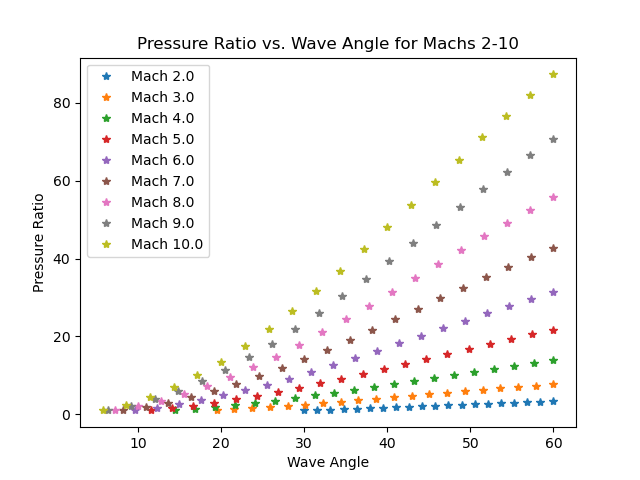
\includegraphics[scale=1.0]{../../images/problem_1/pr_vs_beta_2D.png}
    \caption{Pressure Ratio vs. Beta}
    \label{pr_2d}
\end{figure}

Figure \ref{3d_scatter} shows a 3D scatterplot of the same data in figure \ref{pr_2d}.
The 3D visualization hints at the shape of a response surface relationship between pressure ratio, \(\beta\), and \(M_{1,\infty}\).
Calculation of analytical sensitivities for highly complex non-linear relationships such as these can be difficult, but developing response models can be useful for design of high-speed flow components such as inlets and nozzles.
Despite the greatly increased pressure ratios for a single high-Mach oblique shock, the total pressure recovery associated with such strong single-shock systems is great and should be avoided by replacing the strong shock with a series of weaker shocks.

\begin{figure}[h!]
    \centering
    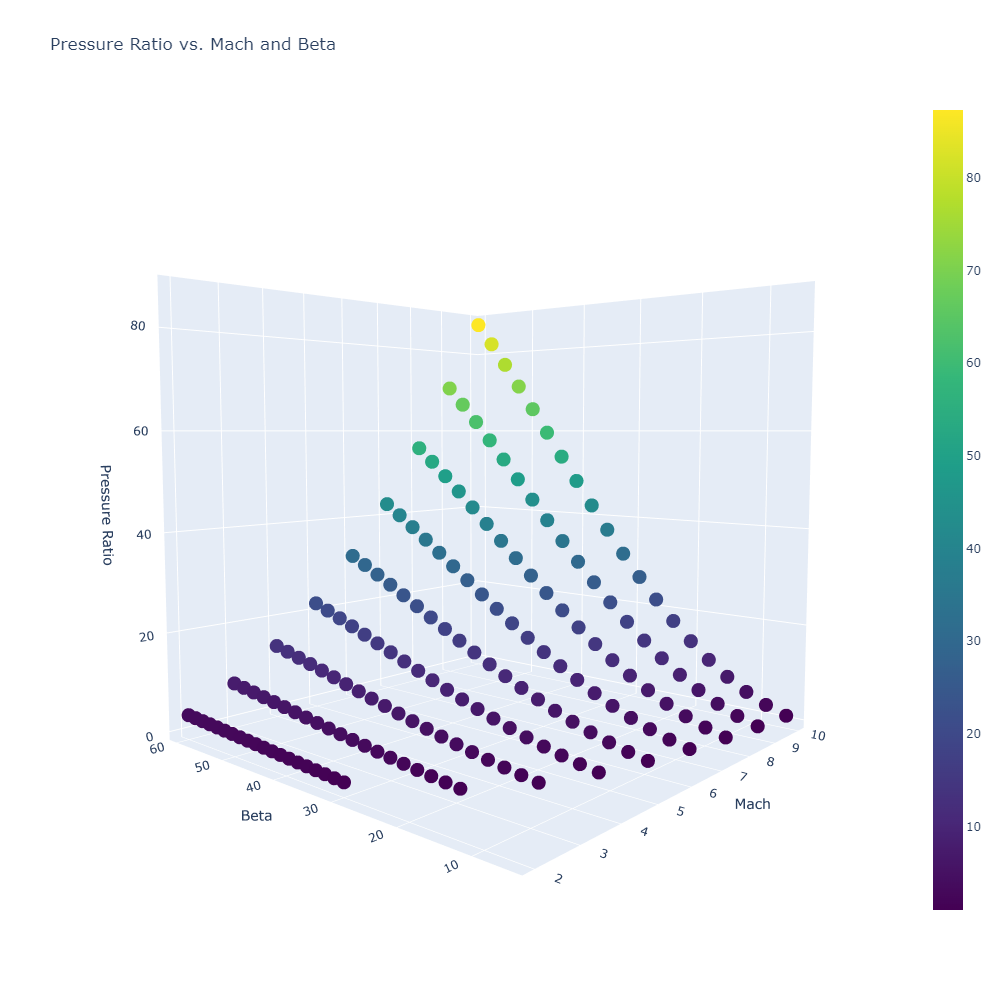
\includegraphics[scale=0.5]{../../images/problem_1/scatter_3d.png}
    \caption{Pressure Ratio vs. Beta and Mach}
    \label{3d_scatter}
\end{figure}

\end{document}